%\documentclass{acm_proc_article-sp}
%\documentclass{sig-alternate}
\documentclass[conference]{IEEEtran}

%\usepackage{fancyheadings}
%\documentclass[times, 10pt,twocolumn]{article}
%\documentclass[conference]{IEEEtran-website}
%\usepackage{latex8}

\usepackage{algorithmic}
\usepackage{multirow}
\usepackage{amssymb, amsmath}
\usepackage{xspace}
\usepackage{times}
\usepackage{graphicx}
\usepackage{epsf}
\usepackage{verbatim}
%\usepackage{psfig}
\usepackage{cite}
\usepackage{url}
\usepackage{color}
\usepackage{alltt}

\newcommand{\StateProjection}{static analysis}
\newcommand{\CurAspectJSubjectCount}{12}

\newcommand{\Add}{\CodeIn{add}}
\newcommand{\AVTree}{\CodeIn{AVTree}}
\newcommand{\Assignment}[3]{$\langle$ \Object{#1}, \Object{#2}, \Object{#3} $\rangle$}
\newcommand{\BinaryTreeRemove}{\CodeIn{BinaryTree\_remove}}
\newcommand{\BinaryTree}{\CodeIn{BinaryTree}}
\newcommand{\Caption}{\caption}
\newcommand{\Char}[1]{`#1'}
\newcommand{\CheckRep}{\CodeIn{checkRep}}
\newcommand{\ClassC}{\CodeIn{C}}
\newcommand{\CodeIn}[1]{{\small\texttt{#1}}}
\newcommand{\CodeOutSize}{\scriptsize}
\newcommand{\Comment}[1]{}
\newcommand{\Ensures}{\CodeIn{ensures}}
\newcommand{\ExtractMax}{\CodeIn{extractMax}}
\newcommand{\FAL}{field-ordering}
\newcommand{\FALs}{field-orderings}
\newcommand{\Fact}{observation}
\newcommand{\Get}{\CodeIn{get}}
\newcommand{\HashSet}{\CodeIn{HashSet}}
\newcommand{\HeapArray}{\CodeIn{HeapArray}}
\newcommand{\Intro}[1]{\emph{#1}}
\newcommand{\Invariant}{\CodeIn{invariant}}
\newcommand{\JUC}{\CodeIn{java.\-util.\-Collections}}
\newcommand{\JUS}{\CodeIn{java.\-util.\-Set}}
\newcommand{\JUTM}{\CodeIn{java.\-util.\-TreeMap}}
\newcommand{\JUTS}{\CodeIn{java.\-util.\-TreeSet}}
\newcommand{\JUV}{\CodeIn{java.\-util.\-Vector}}
\newcommand{\JMLPlusJUnit}{JML+JUnit}
\newcommand{\Korat}{Korat}
\newcommand{\Left}{\CodeIn{left}}
\newcommand{\Lookup}{\CodeIn{lookup}}
\newcommand{\MethM}{\CodeIn{m}}
\newcommand{\Node}[1]{\CodeIn{N}$_#1$}
\newcommand{\Null}{\CodeIn{null}}
\newcommand{\Object}[1]{\CodeIn{o}\ensuremath{_#1}}
\newcommand{\PostM}{\MethM$_{post}$}
\newcommand{\PreM}{\MethM$_{pre}$}
\newcommand{\Put}{\CodeIn{put}}
\newcommand{\Remove}{\CodeIn{remove}}
\newcommand{\RepOk}{\CodeIn{repOk}}
\newcommand{\Requires}{\CodeIn{requires}}
\newcommand{\Reverse}{\CodeIn{reverse}}
\newcommand{\Right}{\CodeIn{right}}
\newcommand{\Root}{\CodeIn{root}}
\newcommand{\Set}{\CodeIn{set}}
\newcommand{\State}[1]{2^{#1}}
\newcommand{\TestEra}{TestEra}
\newcommand{\TreeMap}{\CodeIn{TreeMap}}

\newenvironment{CodeOut}{\begin{scriptsize}}{\end{scriptsize}}
\newenvironment{SmallOut}{\begin{small}}{\end{small}}

\newcommand{\pairwiseEquals}{PairwiseEquals}
\newcommand{\monitorEquals}{MonitorEquals}
%\newcommand{\monitorWField}{WholeStateW}
\newcommand{\traverseField}{WholeState}
\newcommand{\monitorSMSeq}{ModifyingSeq}
\newcommand{\monitorSeq}{WholeSeq}

\newcommand{\IntStack}{\CodeIn{IntStack}}
\newcommand{\UBStack}{\CodeIn{UBStack}}
\newcommand{\BSet}{\CodeIn{BSet}}
\newcommand{\BBag}{\CodeIn{BBag}}
\newcommand{\ShoppingCart}{\CodeIn{ShoppingCart}}
\newcommand{\BankAccount}{\CodeIn{BankAccount}}
\newcommand{\BinarySearchTree}{\CodeIn{BinarySearchTree}}
\newcommand{\LinkedList}{\CodeIn{LinkedList}}

\newcommand{\Book}{\CodeIn{Book}}
\newcommand{\Library}{\CodeIn{Library}}

\newcommand{\Jtest}{Jtest}
\newcommand{\JCrasher}{JCrasher}
\newcommand{\Daikon}{Daikon}
\newcommand{\JUnit}{JUnit}

\newcommand{\trie}{trie}

\newcommand{\Perl}{Perl}


\newcommand{\SubjectCount}{11}
\newcommand{\DSSubjectCount}{two}

\newcommand{\Equals}{\CodeIn{equals}}
\newcommand{\Pairwise}{PairwiseEquals}
\newcommand{\Subgraph}{MonitorEquals}
\newcommand{\Concrete}{WholeState}
\newcommand{\ModSeq}{ModifyingSeq}
\newcommand{\Seq}{WholeSeq}
\newcommand{\Aeq}{equality}

\newcommand{\Meaning}[1]{\ensuremath{[\![}#1\ensuremath{]\!]}}
\newcommand{\Pair}[2]{\ensuremath{\langle #1, #2 \rangle}}
\newcommand{\Triple}[3]{\ensuremath{\langle #1, #2, #3 \rangle}}
\newcommand{\SetSuch}[2]{\ensuremath{\{ #1 | #2 \}}}
%\Comment{
%\newtheorem{definition}{Definition}
%\newtheorem{theorem}[definition]{Theorem}
%}
\newcommand{\Equiv}[2]{\ensuremath{#1 \EquivSTRel{} #2}}
\newcommand{\EquivME}{\Equiv}
\newcommand{\EquivST}{\Equiv}
\newcommand{\EquivSTRel}{\ensuremath{\cong}}
\newcommand{\Redundant}[2]{\ensuremath{#1 \lhd #2}}
\newcommand{\VB}{\ensuremath{\mid}}
\newcommand{\MES}{method-entry state}

\newcommand{\Small}[1]{{\small{#1}}}

\newcommand{\CenterCell}[1]{\multicolumn{1}{c|}{#1}}
\newcommand{\Fix}[1]{{\large\textbf{FIX}}#1{\large\textbf{FIX}}}

\newcommand{\CodeInS}[1]{{\scriptsize\texttt{#1}}}
\newcommand{\CodeInFN}[1]{{\footnotesize\texttt{#1}}}
\newcommand{\CodeOutFN}{\footnotesize}

\newcommand{\SmallSpace}{\vspace*{-1.4ex}}
\newcommand{\Item}{\SmallSpace\item}
\newenvironment{Itemize}{\begin{itemize}}{\end{itemize}\SmallSpace}
\newenvironment{Enumerate}{\begin{enumerate}}{\end{enumerate}\SmallSpace}

\newtheorem{definition}{Definition}
\newtheorem{theorem}[definition]{Theorem}

%\newcommand{\Item}{\vspace*{-0.5ex}\item\vspace*{-0.5ex}}
%\newenvironment{Itemize}{\begin{itemize}\vspace*{-1ex}}{\end{itemize}\vspace*{-1ex}}
%\newenvironment{Enumerate}{\begin{enumerate}\vspace*{-1ex}}{\end{enumerate}\vspace*{-1ex}}
\newenvironment{Definition}{\begin{definition}\vspace*{-1.5ex}}{\end{definition}\vspace*{-1.5ex}}

% Local Variables:
% mode:latex
% End:


\usepackage{indentfirst}
\usepackage{listings, algorithm, algorithmic, graphicx, listing}
\usepackage{color}
\usepackage{ulem}
\usepackage{url}
\usepackage{xspace}

\newcommand{\ie}{i.e.}
\newcommand{\eg}{e.g.}
\newcommand{\ea}{et al.\xspace}
\newcommand{\aka}{a.k.a.}

\newcommand{\errors}{14 }
\newcommand{\crash}{9 }
\newcommand{\noncrash}{5 }
\newcommand{\topnum}{10 }
\newcommand{\subjectnum}{5 }
\newcommand{\avgrank}{7 }

\newcommand{\avgtime}{4 }

\newcommand{\randoop}{Randoop\xspace}
\newcommand{\weka}{Weka\xspace}
\newcommand{\jchord}{JChord\xspace}
\newcommand{\synoptic}{Synoptic\xspace}
\newcommand{\soot}{Soot\xspace}

\newcommand{\tool}[1]{#1}
\newcommand{\FailureDoc}{\tool{Failure\-Doc}\xspace}
\newcommand{\ourtool}{\tool{Conf\-Diagnoser}\xspace}
\newcommand{\smallstep}{\relax}
\newcommand{\tinystep}{\relax}

% Add line between figure and text
\makeatletter
\def\topfigrule{\kern3\p@ \hrule \kern -3.4\p@} % the \hrule is .4pt high
\def\botfigrule{\kern-3\p@ \hrule \kern 2.6\p@} % the \hrule is .4pt high
\def\dblfigrule{\kern3\p@ \hrule \kern -3.4\p@} % the \hrule is .4pt high
\makeatother \addtolength{\textfloatsep}{-.5\textfloatsep}
\addtolength{\dbltextfloatsep}{-.5\dbltextfloatsep}
\addtolength{\floatsep}{-.5\floatsep}
\addtolength{\dblfloatsep}{-.5\dblfloatsep}

%\newcommand{\CodeIn}[1]{{\small\texttt{#1}}}
\newcommand{\edit}[2]{\sout{#1}{#2}}

%\newcommand{\ie}{i.e.}
%\newcommand{\eg}{e.g.}
%\newcommand{\ea}{et al.\xspace}
%\newcommand{\aka}{a.k.a.}

% \|name| or \mathid{name} denotes identifiers and slots in formulas
\def\|#1|{\mathid{#1}}
\newcommand{\mathid}[1]{\ensuremath{\mathit{#1}}}
% \<name> or \codeid{name} denotes computer code identifiers
\def\<#1>{\codeid{#1}}
\newcommand{\codeid}[1]{\ifmmode{\mbox{\ttfamily{#1}}}\else{\ttfamily #1}\fi}

\newcommand{\cut}[1]{}
\newcommand{\todo}[1]{{\bfseries [[{#1}]]}}

\newcommand{\ttlcb}{\texttt{\char "7B}}
\newcommand{\ttrcb}{\texttt{\char "7D}}

\newcommand{\phz}{\phantom{0}}

\begin{document}
\normalem

%\title{Explaining Software Configuration Problems}
\title{Automated Software Configuration Error Diagnosis} % \\ for Java Software}
%\subtitle{xx}

%\author{\IEEEauthorblockN{Sai Zhang \quad Michael D. Ernst}
%\author{\IEEEauthorblockN{Sai Zhang}
%\IEEEauthorblockA{University of Washington\\
%szhang@cs.washington.edu} \and \IEEEauthorblockN{Cheng
%\IEEEauthorblockA{Shanghai Jiao Tong University\\
%cheng.zhang.stap@sjtu.edu.cn} 
%}


%\numberofauthors{1}
%\author{
%\alignauthor Sai Zhang \quad Michael D. Ernst\\
%       \affaddr{Department of Computer Science \& Engineering}\\
%       \affaddr{University of Washington, USA}\\
%       \email{\{szhang,  mernst\}@cs.washington.edu}
%}
\author{\IEEEauthorblockN{Sai Zhang \quad Michael D. Ernst}
\IEEEauthorblockA{Department of Computer Science \& Engineering\\
University of Washington, USA\\
\{szhang,  mernst\}@cs.washington.edu}}


\maketitle \sloppy

\begin{abstract}

The behavior of a software system often depends on how that system is
configured. 
Small configuration errors can lead to
hard-to-diagnose undesired behaviors.
We present a technique (and its tool implementation,
called \ourtool) to identify the root cause of a configuration error ---
a single configuration option that can be changed to produce desired behavior.
Our technique uses static analysis,
dynamic profiling, and statistical analysis to link the
undesired behavior to specific configuration options.
It differs from existing approaches in
two key aspects: it does not
require users to provide a testing oracle (to check whether
the software functions correctly) and thus is fully-automated; and it can
diagnose both crashing and non-crashing
errors.

%, and uses statistical inference to link the observed
%undesired behaviors to specific configuration options.

%$\blacksquare$ say a few of our tool's technique


%We have built a tool called \ourtool for Java software.
We evaluated \ourtool on \noncrash non-crashing configuration errors
and \crash crashing configuration errors from
\subjectnum configurable software systems written in Java.
On average, the root cause was \ourtool's fifth-ranked suggestion; in
\topnum out of \errors errors, the root cause was the top 3 suggestions;
and more
than half of the time, the root cause was the first suggestion.

% \ourtool identifies the
% source of the misconfiguration
% as the top 3 root cause for \topnum out of all \errors errors,
% making it a promising solution. %in automated debugging. %error diagnosis. %alternative to manual debugging.

%that xxx -- \ourtool uses these
%xxx to link the undesired behavior to specific configuration options. Our
%results using \ourtool to solve misconfigurations in xxx, xxx, xxx show
%that \ourtool identifies the soruce of the misconfiguration xxxx.

%\todo{Add this somewhere in the abstract:  Our technique uses static analysis,
%dynamic profiling, and statistical analysis to link the
%undesired behavior to specific configuration options.}

\end{abstract}

\label{fake-label-for-etags}


\section{Introduction}
\label{sec:introduction}

Many software applications support
configuration options that allow users to
customize their behavior. This flexibility has a cost: when something
goes wrong, diagnosing a configuration error can be both time-consuming
and frustrating. Technical support contributes 17\% of the total cost of ownership of
today's software, and troubleshooting misconfigurations
is a large part of technical support~\cite{confevidence}.

Software misconfigurations may lead to incorrect output (i.e., non-crashing
errors) or to unexpected termination
(i.e., crashing errors).  Even when an application outputs an error
message, it is often cryptic or misleading~\cite{Yin:2011:ESC, Attariyan:2010:ACT, Hubaux:2012, rangefix}.
Users may not even think of configuration as a cause of their problem.
% Thus, users must search manuals, FAQs, and online forums to find potential
% solutions.% to the problem. %$\blacksquare$ this process is frustrating..
\looseness=-1

\subsection{Motivating Example}
\label{sec:mot}

%This section describes a real scenario in which we used \ourtool to solve %a configuration problem. 
We next describe a real scenario in which we used \ourtool to solve a configuration problem. 
We received a ``bug report'' against the Randoop
automated test generation tool~\cite{PachecoLET2007},
from a testing expert who had been using Randoop for quite a while.
The ``bug report'' indicated that Randoop terminated normally but
failed to generate tests for the NanoXML~\cite{nanoxml} program. 
%The symptom is that
%Randoop terminates normally but does not generate any tests.
%on NanoXML, it 

Although the reported problem is deterministic and fully reproducible,
it is a silent, non-crashing failure and is
challenging to diagnose. Differing from
a crashing error, Randoop did not exhibit a crashing point, dump
 a stack trace, output an error message, or indicate suspicious program
variables that may have incorrect values. Lacking such information
makes many
techniques such as dynamic slicing~\cite{Zhang:2003:PDS},
dynamic information flow tracking~\cite{Attariyan:2010:ACT}, and
failure trace analysis~\cite{Rabkin:2011:PPC} inapplicable.
In addition, for this scenario, the person who reported the bug had already
minimized the bug report:  if any part of the 
configuration or input is removed, Randoop either crashes or
no longer exhibits this error.
This further makes 
search-based fault isolation techniques such as delta debugging~\cite{Zeller:2002:ICC}
ineffective.
\looseness=-1

%there is no obvious testing oracle\todo{Why
%  not?  Wouldn't ``some output vs.\ no output'' be a testing oracle?} to check whether
%Randoop behaves as desired, which  Moreover, 

In fact, this bug report does not reveal a real bug
in the Randoop code. Its root cause is that
the user failed to set one configuration option.
Despite the simplicity of the solution, to the best of our knowledge, no
previous configuration error diagnosis technique~\cite{Attariyan:2008:UCD, 
Whitaker:2004:CDS, Wang:2004:AMT,
Attariyan:2010:ACT, Rabkin:2011:PPC, autoflow, failuredoc} can be directly applied.


%We reproduce this problem in a \ourtool-enabled environment.
%It determines which predicates exemplify the buggy behaviors.


\begin{figure}[t]
\begin{CodeOut}
\begin{alltt} 
Suspicious configuration option: maxsize

It affects the behavior of predicate:
"newSequence.size() > GenInputsAbstract.maxsize"
(line 312, class: randoop.ForwardGenerator) 

This predicate evaluates to true:
  3.3\% of the time in normal runs (3830 observations)
  32.5\% of the time in the undesired run (2898 observations)
\end{alltt}
\end{CodeOut}
\vspace*{-13pt}
\Caption{{\label{fig:output}
The top-ranked configuration option in \ourtool's error report
for the motivating example in Section~\ref{sec:mot}. 
}} \vspace{-1mm}
\end{figure}
%, this predicate evaluates to true:   (1315 observation%run, it evaluates to true:  (2727 observations)s)

As an alternative, we can use our technique (and its tool implementation \ourtool)
to diagnose and correct this problem. We first reproduced the
error in a \ourtool-instrumented Randoop version, then \ourtool
diagnosed the error's root cause by analyzing the recorded execution profile.
\ourtool produced
a report (Figure~\ref{fig:output}) in the form of an ordered list of
suspicious configuration options that should be inspected.
The error report in Figure~\ref{fig:output} suggests that
a configuration option named
\CodeIn{maxsize} is the most likely one.
The report also provides relevant 
information to explain why: % about the reason why \CodeIn{maxsize} should be account for:
a program predicate affected by \CodeIn{maxsize} behaves dramatically
differently between the recorded undesired execution
and the correct executions found in \ourtool's database.
\looseness=-1

Figure~\ref{fig:example} shows the relevant code snippet
in Randoop.  When Randoop generates a new test (line 100, in the form of
a method-call sequence),
Randoop compares its length with \CodeIn{maxsize}
(default value: 100). If the
generated sequence's length exceeds this pre-defined limit,
Randoop discards it to avoid length explosion in further
test generation.
Although \CodeIn{maxsize}'s default value was carefully chosen
by the Randoop developers
and works well for many programs (including those used to test
Randoop during its development), the generated sequences for NanoXML
are much longer than usual and using \CodeIn{maxsize}'s default value
results in 32.5\% of the generated sequences being discarded
(including sequences that the user wishes to retain).
\ourtool captures such abnormal behavior from Randoop's
silent failure, pinpoints the
\CodeIn{maxsize} option, and suggests the user to change its value.
The problem is resolved if
the user changes \CodeIn{maxsize} to a larger value, for example 1000.
\looseness=-1


%Guided by the report, we can further find out
%the root cause of Randoop's silent failure
%is because 

%and only 14.4\% of the generated sequences have been discarded.
%However,

%are discarded because the generated sequences are much longer.  

\begin{figure}[t]
%\vspace{-2mm}
\vspace{1mm}
\small{In class: randoop.main.GenInputsAbstract}\\
%\small{//a configuration option to control a sequence's max length}
\vspace{-5mm}
\begin{CodeOut}
\begin{alltt}
     //{The maxsize configuration option. Default value: 100.}
157. public static int maxsize = readFromCommandLine(); 
\end{alltt}
\end{CodeOut}

{\small{In class: randoop.ForwardGenerator}}\\
\vspace{-5mm}
\begin{CodeOut}
\begin{alltt}
99.  public ExecutableSequence step() \ttlcb
100.   ExecutableSequence eSeq = createNewUniqueSequence();
101.   AbstractGenerator.currSeq = eSeq.sequence;
102.   eSeq.execute(executionVisitor);
103.   processSequence(eSeq);
104.   if (eSeq.sequence.hasActiveFlags()) \ttlcb
105.     componentManager.addGeneratedSequence(eSeq.sequence);
106.   \ttrcb
107.   return eSeq;
108. \ttrcb

310. private ExecutableSequence createNewUniqueSequence() \ttlcb
311.   Sequence newSequence = ...; //create a sequence
312.   if (newSequence.size() > GenInputsAbstract.maxsize) \ttlcb
313.     return null;
314.   \ttrcb
315.   if (this.allSequences.contains(newSequence)) \ttlcb
316.     return null;
317.   \ttrcb
318.   return new ExecutableSequence(newSequence);
319. \ttrcb
\end{alltt}
\end{CodeOut}
\tinystep
\vspace*{-3.0ex} \Caption{{\label{fig:example} 
Simplified code excerpt from Randoop~\cite{PachecoLET2007}
corresponding to the configuration problem reported in Figure~\ref{fig:output}.
%\todo{Need line number for \<int maxsize = ...> line at top.}
%A forward slice computed by the traditional slicing algorithm~\cite{Horwitz:1988:ISU}
%from the seed statement includes statements 2, 3,
%4, 5, 6, 7, 9, 13, 14, 16, 17, and 19.
%By contrast, a thin slice~\cite{Sridharan:2007}
%only contains line 13.
}} \vspace{-1mm}
\end{figure}




%\vspace{1mm}
%\noindent \textbf{\textit{Our technique.}} 

\subsection{Diagnosing Configuration Errors}

Correcting a configuration error can be divided into two
separate tasks: identifying which specific configuration option is
responsible for the unexpected behavior, and determining a better value for
the configuration option. This paper addresses the former task: finding
the root cause of a configuration error.
%, and leave the later task
%of fixing


%The goal of \textbf{our technique} is to help users find solutions to the configuration
%problems they are facing.  
Our technique is designed to be used by system administrators
and end-users when they encounter an error
that they do not know how to fix. It uses three steps to 
link the undesired behavior to specific root cause configuration options:

\begin{itemize}
\item \textbf{Configuration Propagation Analysis}. For
each configuration option, \ourtool
uses a lightweight dependence analysis, called thin slicing~\cite{Sridharan:2007},
to statically identify the predicates it affects in the source code.

\item \textbf{Configuration Behavior Profiling}. \ourtool
selectively instruments the program-to-diagnose
so that it records the run-time behaviors of affected predicates
in an execution profile.
%diagnosed code when undesired behavior
%is observed.
When the user encounters a suspected configuration error, the user
reproduces the error using the instrumented version of the program.

\item \textbf{Configuration Deviation Analysis}.
\ourtool selects, from a pre-built database, correct execution profiles that are as
similar as possible to the undesired one.
Then, it identifies the predicates whose dynamic behaviors deviate the most
between correct and undesired executions.
The behavioral differences in the recorded predicates provide evidence for
what predicates in a program might be behaving
abnormally and why. %This helps to further reason about its root cause.
For each deviated predicate, \ourtool further identifies
its affecting configuration options as the likely root causes.
Finally, it outputs a ranked list of suspicious configuration options and explanations.
% (between
%the undesired execution and the selected correct executions).

\end{itemize}

%\ourtool  Once a \ourtool user encounter an unexpected
%behavior, she can reproduce the problem on a \ourtool-enabled environment,
%where \ourtool monitors the program execution. 

%The output of \ourtool is a ranked list of
%configurations that could possibly account for
%those deviated predicates, and should be checked
%by users.

An important component in \ourtool is the pre-built
database, which contains profiles
from known correct executions. We envision that 
the software developers build this database at release time.
The database can be
further enriched by software users as more correct
executions are accumulated. 
In our experiments (Section~\ref{sec:evaluation}), we
built a database of 6--16 execution profiles by running examples from software
user manuals, FAQs, discussion mailing list,
forum posts, and published papers.  We
found that even such a small database worked remarkably
well for error diagnosis.

Compared to previous approaches~\cite{Zeller:2002:ICC, Zhang:2003:PDS,
Rabkin:2011:PPC, Whitaker:2004:CDS, Attariyan:2010:ACT, Wang:2004:AMT}, \ourtool has
several notable features:

\begin{itemize}
\item \textbf{It is fully automated}.
\ourtool does not require a user to specify
\textit{when}, \textit{why}, or \textit{how} the program fails. This is
different than many well-known automated debugging techniques such
as delta debugging~\cite{Zeller:2002:ICC}, information flow analysis~\cite{Attariyan:2010:ACT},
 and dynamic slicing~\cite{Zhang:2003:PDS}.
Our technique also provides an \emph{explanation} of
why a configuration option is suspicious. 

\item \textbf{It can diagnose both non-crashing and crashing errors}.
Most previous techniques~\cite{Rabkin:2011:PPC,
Whitaker:2004:CDS, Attariyan:2010:ACT, Su:2007:AIC} focus exclusively on configuration errors
that cause a crash, an error message, or a stack trace.
By contrast, \ourtool diagnoses
configuration problems that manifest themselves as
either visible or silent failures.

\item \textbf{It requires no OS-level support.} Our technique requires no alterations to
the JVM or standard library. This distinguishes our work from
competing techniques such as OS-level configuration
error troubleshooting~\cite{Whitaker:2004:CDS, Su:2007:AIC}.% or dynamic taint tracking~\cite{clause07july}.

\end{itemize}

%\ourtool is designed to help users find solutions to the configuration
%problems they are facing.  


%When a configuration error happens, users can
%use \ourtool to diagnose the problem based on the recorded profile.

%\ourtool is run offline, once erroneous
%behavior has been observed. A \ourtool user reproduces
%the problem by executing the application while \ourtool attaches to
%the executing application processes and monitors xxx.

%We envision that \ourtool can be used by end-users or
%administrators t
%When an end-user or administrator wishes to diagnose a


%The instrumented version is deployed on the user side to collect program execution
%profiles (including both good and bad runs). When the user finds the program
%does not work as expected on a given input and configurations,
%he/she can invoke the Configuration Deviation Analysis component (Section~\ref{sec:analysis}) to
%diagnose the observed behavior. Our technique's output is a ranked list of
%configurations that could possibly explain the why the program does not produce the desirable result. Those
%configurations, if changed, may even fix the unexpected behavior.



%the software developers
%built the database initially, and other users can also enrich
%the database.
%, a
%the software developers provide a profile database, which users can use
%to query. The users can also enrich the database, providing their
%own examples. even a single run

%use the recorded profile message to query this database, perhaps via a web
%service.
 
%The core of our approach is to xxx. 
%We envision this being done by the developers
%at release time. 

%this technique xxx could be performed by
%the software developers; users would need only to provide
%the profiles xxx to back a diagnosis.


%We have developed a tool, called \ourtool, that uses xxx



\begin{figure*}[!]
  \centering
  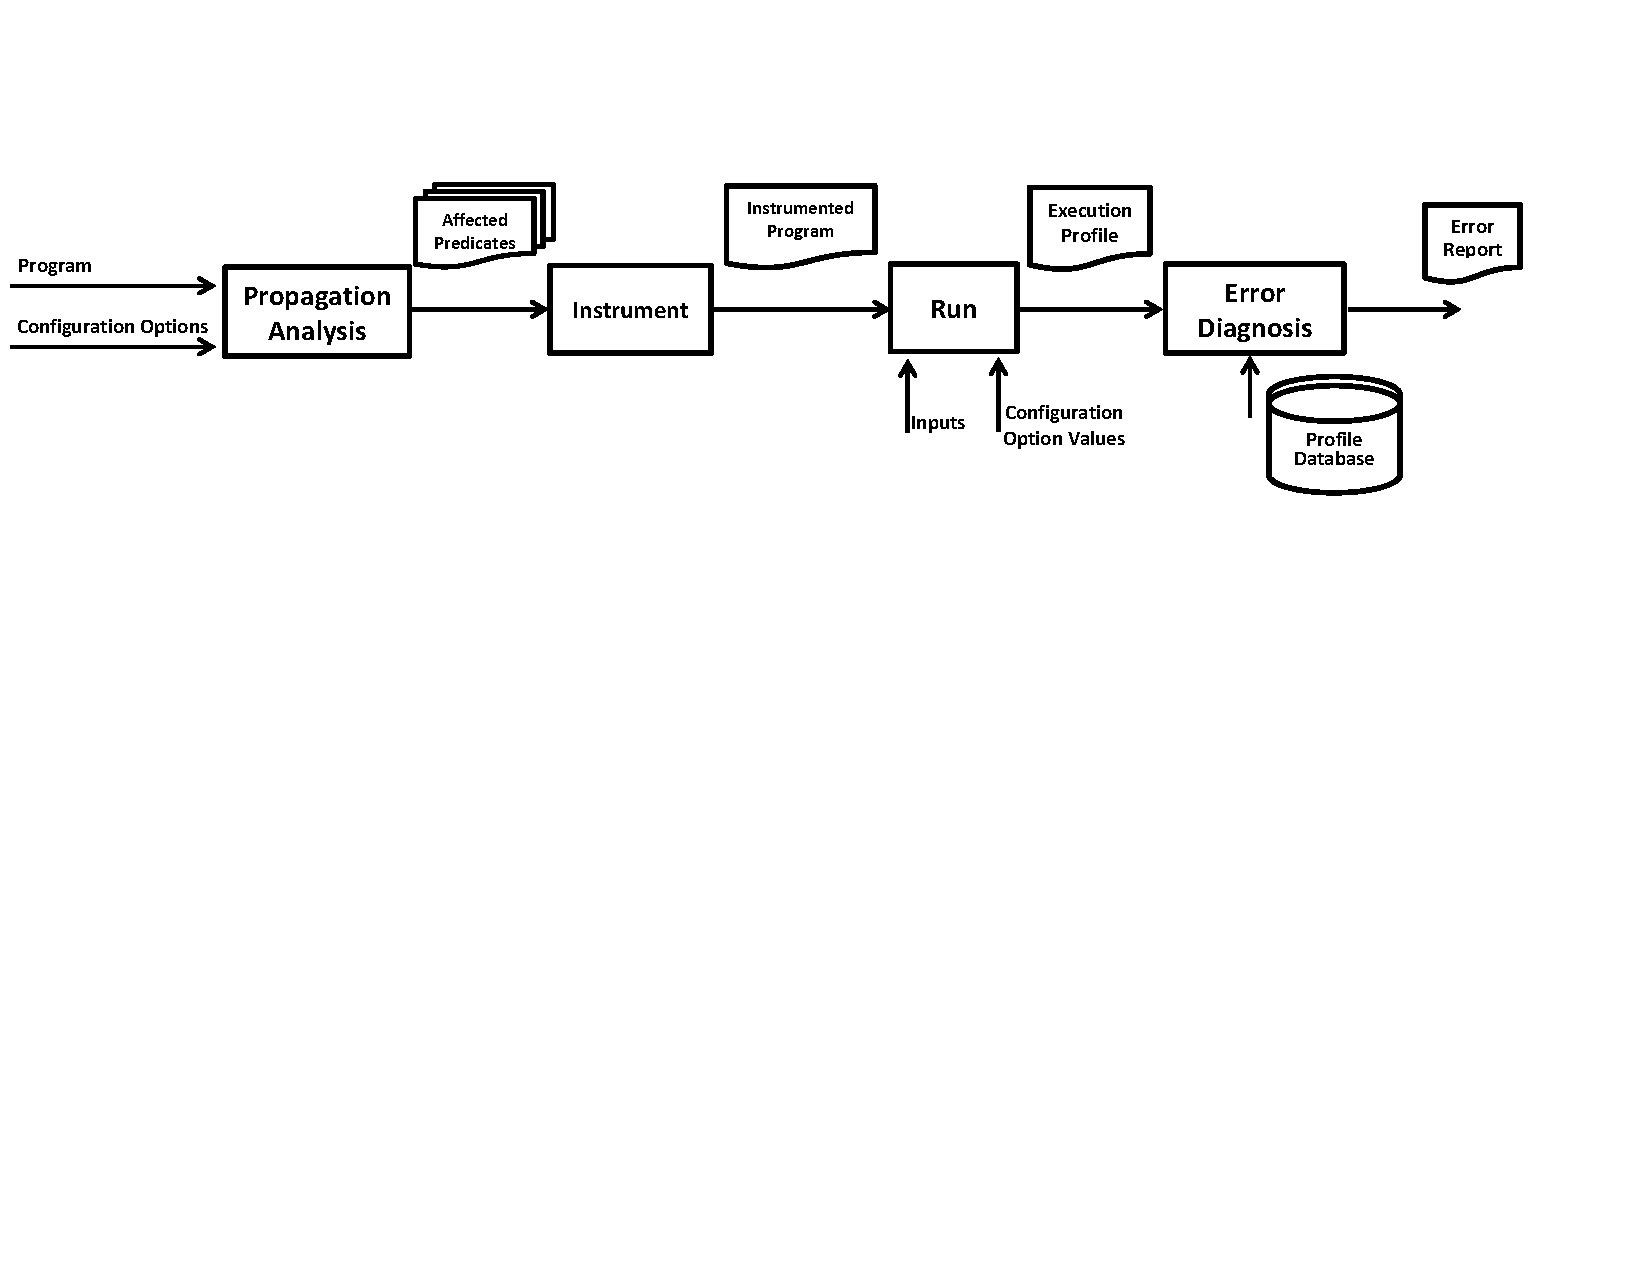
\includegraphics[scale=0.600]{architecture}
  \vspace*{-2.0ex}\caption {{\label{fig:workflow} The workflow of our configuration error diagnosis technique.
``Propagation Analysis'' is described in Section~\ref{sec:prop}.
The ``Instrument'' and ``Run'' components correspond to the Configuration Behavior Profiling step in Section~\ref{sec:profiling}.
``Deviation Analysis'' is described in Section~\ref{sec:analysis}.
}}
%\todo{The paper sometimes uses the terminology ``execution profile'' and
%  sometimes ``trace''.  Please be consistent.  I like ``execution profile''
%  better, because there is no temporal information about ordering in it.}
%\todo{The use of ``inputs'', in this figure and elsewhere, suggests that
%  the user runs multiple executions.  In fact, it is one execution, right?
%  I would change the arrow label ``inputs'' to ``input'' and
%  ``configurations'' to ``configuration''.  I would also label them as
%  ``bad runs''.  Then, I would change the database symbol's label from
%  ``Profile Database'' to ``Profile Database (good runs)''.}
\end{figure*}

\label{dummy-for-etags-workflow}


%\vspace{1mm}
%\noindent \textbf{\textit{Evaluations.}} 

\subsection{Evaluation}

We evaluated \ourtool on \errors real configuration errors
(\crash crashing errors and \noncrash non-crashing errors)
from \subjectnum projects.
On average, \ourtool's 5th report was the root cause; in
\topnum out of \errors cases, the root cause was \ourtool's
top 3 reports; and in over half of all
cases, the root cause was \ourtool's first report.
% This permits \ourtool user to focus on a few specific configuration
% options when deciding how to fix the problem. 
Assuming the database of correct execution profiles already exists,
\ourtool takes less than \avgtime minutes on average to diagnose
one error.  \ourtool's accuracy and speed make it an attractive alternative
to manual debugging.

%\todo{Defer most or all of the below details, especially ones related to
%  internal implementation choices.  This is too many low-level details at
%  this point in the paper.}

We compared \ourtool to a previous technique, called ConfAnalyzer~\cite{Rabkin:2011:PPC},
which uses dynamic information flow analysis to reason about the root cause of a
configuration error. \ourtool produced better results for 8 errors,
equivalent results for 3 errors, and worse results for 3 errors.

%As a result, \ourtool produced accurate diagnosis information for the \noncrash
%non-crashing errors that ConfAnalyzer failed to diagnose,
%and produced better or the same results
%for 6 out of the \crash crashing errors. 

We also compared \ourtool to two techniques leveraging
existing fault localization techniques~\cite{Jones:2002, McCamant:2003}
to diagnose configuration errors. 
\ourtool substantially outperformed both of them.

%\todo{Should I add this sentence: suggesting the necessity of
%designing new configuration error diagnosis techniques. Seems a bit
%verbose}
%, suggesting
%the necessity of designing new configuration error diagnosis techniques.% such as \ourtool.

%three variants and one existing
%technique, .
%The three variants is based on \ourtool, but use different
%abstractions rather than
%the affected predicates as computed by thin slicing in
%error diagnosis. ConfAnalyzer, one of the most precise
%configuration error diagnosis technique, uses dynamic
%Our experimental results show that \ourtool significantly
%outperformed three variants.
%Compared to ConfAnalyzer,



Finally, we evaluated two internal design choices of \ourtool.
First, we show that using thin slicing~\cite{Sridharan:2007} to compute the affected
predicates yielded more accurate diagnosis than using full slicing~\cite{Horwitz:1988}.
Second, we %investigated the effects of varying the comparison execution profiles from \ourtool's database, and
show that varying the execution
profile selection strategy can result in substantially different
results. %, depending on the application being analyzed;
The similarity-based selection strategy used in \ourtool outperformed
the other two strategies.


%\ourtool outputs an ordered list of probable root causes.
%Each entry in the list is a user-settle configuration option;
%our results show that \ourtool typically outputs
%the actual responsible configuration option as the top 3 in the list.

%By finding the
%needle in the haystack, \ourtool can be an attractive ...

%While xxx analysis takes a few minutes for a complex application,
%automated error diagnosis is still considerably faster and
%less labor-intensive than manual debugging or searching
%through other resources.

%$\blacksquare$ our technique is lightweighted.

%\vspace{1mm}
%\noindent \textbf{\textit{Contributions.}}


\subsection{Contributions}
This paper makes the following contributions:

\begin{itemize}
%\item \textbf{Problem.} To the best of our knowledge, we are the first to address
%the invalid thread access error detection problem for multithreaded GUI applications.

\item \textbf{Technique.} We present a technique to diagnose
software configuration errors. Our technique uses static analysis,
dynamic profiling, and statistical analysis to link the
undesired behavior to specific configuration options (Section~\ref{sec:technique}).


\item \textbf{Implementation.} We implemented our technique 
in a tool, called \ourtool, for Java software (Section~\ref{sec:implementation}). It is available at
\url{http://config-errors.googlecode.com}. 


\item \textbf{Evaluation.} We applied \ourtool to diagnose~\errors
configuration errors in \subjectnum
configurable Java software projects. The results
show the usefulness of the proposed technique (Section~\ref{sec:evaluation}).

\end{itemize}




% LocalWords:  misconfigurations NanoXML maxsize newSequence GenInputsAbstract
% LocalWords:  randoop ForwardGenerator pre readFromCommandLine eSeq currSeq
% LocalWords:  ExecutableSequence createNewUniqueSequence AbstractGenerator
% LocalWords:  executionVisitor processSequence componentManager ConfAnalyzer
% LocalWords:  addGeneratedSequence


\section{Technique}
\label{sec:technique}

We model configurations as a set of key-value pairs, where
the keys are strings and the values have arbitrary type. This is a
convenient abstraction for analysis as well as a close match for
many standard configuration APIs. It is the abstraction offered
by the POSIX system environment, the Java Properties API,
and the Windows registry.


Figure~\ref{fig:workflow} sketches the high-level workflow of our technique.
Our technique takes as input a program and a list of configuration options.
It first performs a configuration propagation analysis to identify
program elements (here, using the abstraction of predicates) that might be
affected by each configuration (Section~\ref{sec:prop}). Then, it
instruments the original program (Section~\ref{sec:profiling}).

The instrumented version is deployed on the user side to collect program execution
profiles (including both good and bad runs). When the user finds the program
does not work as expected on a given input and configurations,
he/she can invoke the Configuration Deviation Analysis component (Section~\ref{sec:analysis}) to
diagnose the observed behavior. Our technique's output is a ranked list of
configurations that could possibly explain the why the program does not produce the desirable result. Those
configurations, if changed, may even fix the unexpected behavior.

\begin{figure*}[!]
  \centering
  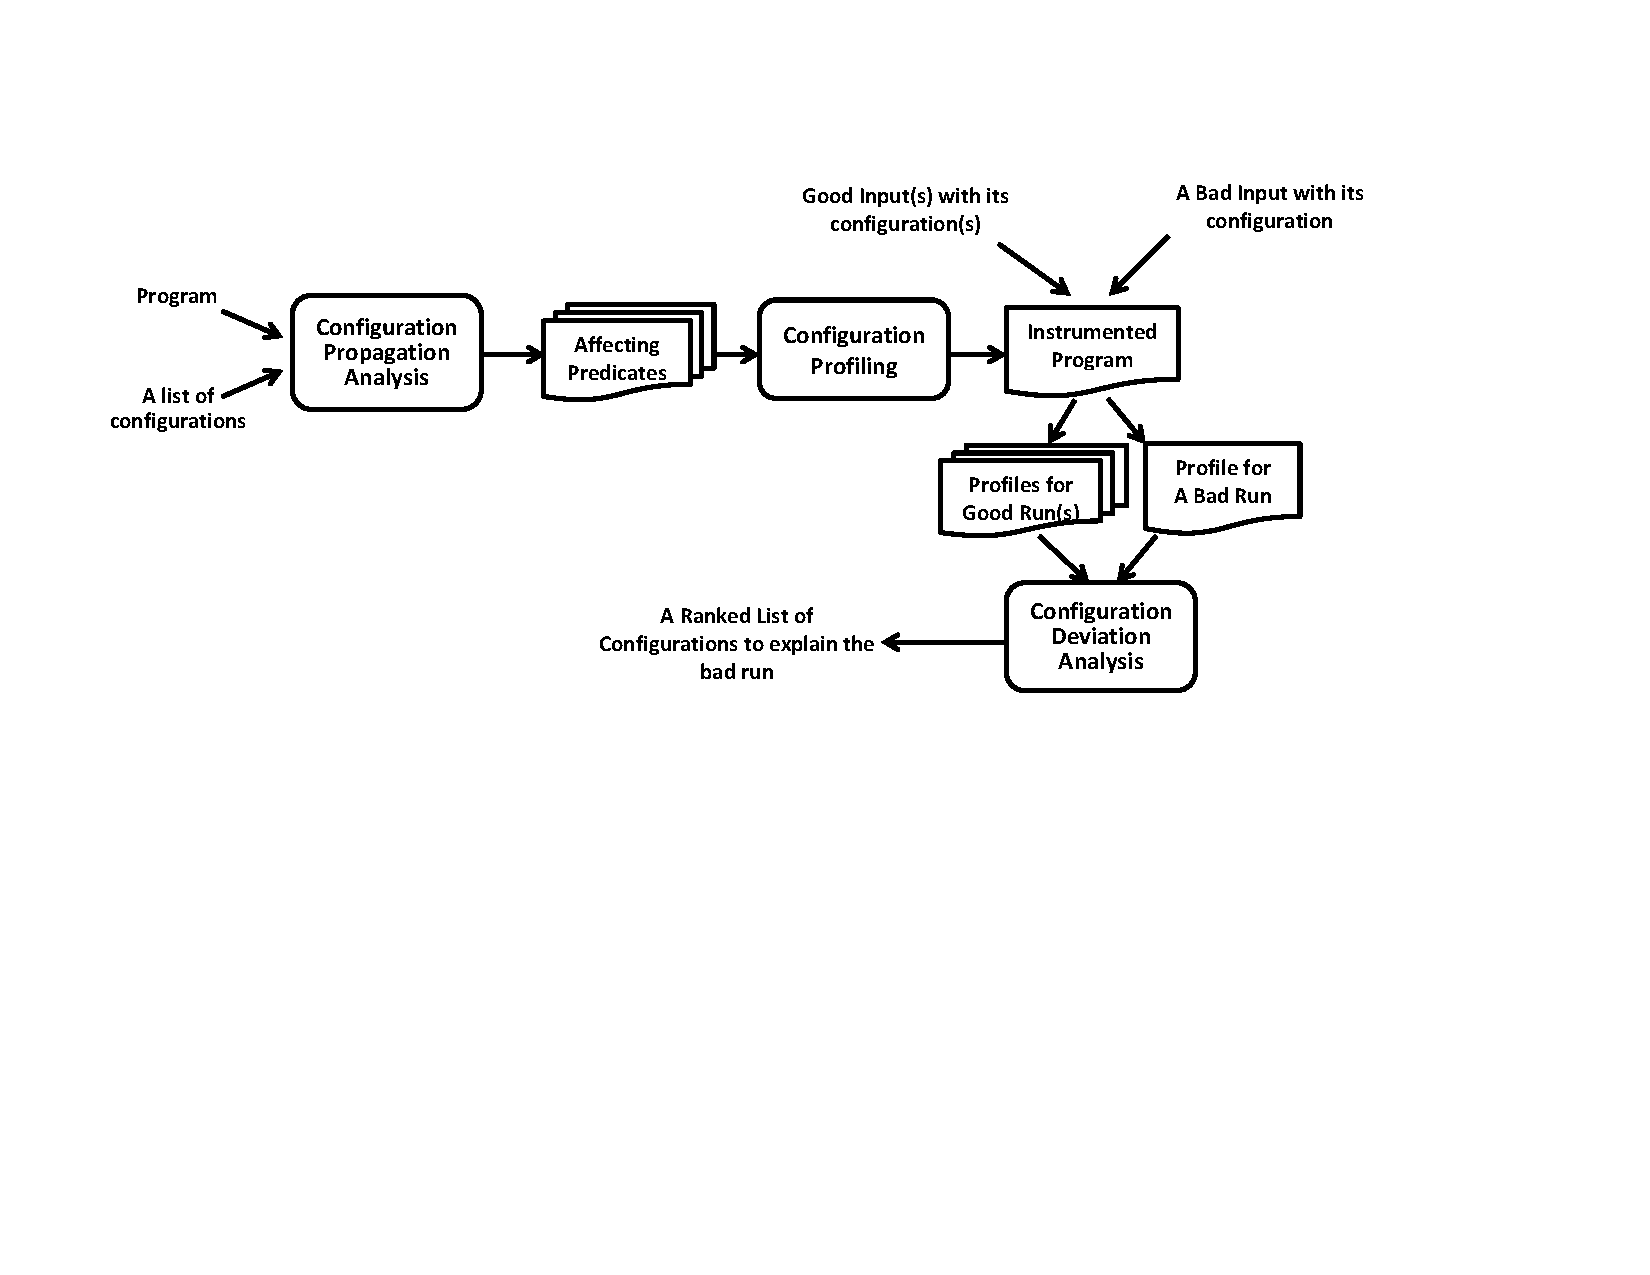
\includegraphics[scale=0.750]{workflow}
  \vspace*{-2.0ex}\caption {{\label{fig:workflow} The workflow of our configuration error explanation technique.
}}
\end{figure*}

\subsection{Configuration Propagation Analysis}
\label{sec:prop}

Given a configuration option, this step statically determines its affected program
elements in the abstraction level of \textit{predicates}. Using predicates
as the abstraction level makes our technique focus on program data flows, instead
of all executed statements.

To identify those affected program predicates, a straightforward way is using program
slicing~\cite{Horwitz:1988:ISU} to compute a forward slice from the assignment statement of the given
configuration option. Unfortunately, traditional slicing includes all statements that
\textit{may} affect a point of interest and often grows too large.

Our technique uses thin slicing~\cite{Sridharan:2007} as a manner to include
\textit{only} statements that are directly affected by the configuration.
We illustrate the advantages of using thin slicing 
 in Figure~\ref{fig:example}.

\begin{figure}[t]
\vspace{-2mm}
\small{//a configuration option to control a sequence's max length}
\vspace{-2mm}
\begin{CodeOut}
\begin{alltt}
int maxsize = readFromCommandLine();  //\textit{seed statement}

1.  public ExecutableSequence step() \ttlcb
2.    ExecutableSequence eSeq = createNewUniqueSequence();
3.    AbstractGenerator.currSeq = eSeq.sequence;
4.    eSeq.execute(executionVisitor);
5.    processSequence(eSeq);
6.    if (eSeq.sequence.hasActiveFlags()) \ttlcb
7.      componentManager.addGeneratedSequence(eSeq.sequence);
8.    \ttrcb
9.    return eSeq;
10. \ttrcb

11. private ExecutableSequence createNewUniqueSequence() \ttlcb
12.   Sequence newSequence = ...; //sequence creation step omitted
13.   if (newSequence.size() > maxsize) \ttlcb
14.     return null;
15.   \ttrcb
16.   if (this.allSequences.contains(newSequence)) \ttlcb
17.     return null;
18.   \ttrcb
19.   return new ExecutableSequence(newSequence);
20. \ttrcb
\end{alltt}
\end{CodeOut}
\tinystep
\vspace*{-3.0ex} \Caption{{\label{fig:example} 
Code excerpt from the Randoop automated test generator~\cite{randoop}.
A forward slice computed by the traditional slicing algorithm~\cite{Horwitz:1988:ISU}
from the seed statement includes statements 2, 3,
4, 5, 6, 7, 9, 13, 14, 16, 17, and 19.
By contrast, a thin slice~\cite{Sridharan:2007}
only contains line 13.
}} %\vspace{-1.8mm}
\end{figure}


\begin{figure}[t]
\begin{CodeOut}
\begin{alltt} 
Configuration option: randoop.main.GenInputsAbstract.maxsize
The predicate: "newSequence.size() > GenInputsAbstract.maxsize" in
"randoop.ForwardGenerator.createNewUniqueSequence()" (line: 312)
shows different behaviors.

In good runs, it evaluates to true:  14.4\% of the time (1315 observations)
In the bad run, it evaluates to true: 32.3\% of the time (2727 observations)

\end{alltt}
\end{CodeOut}
\vspace*{-15pt}
\Caption{{\label{fig:output}
The diagnosis output . The top ranked option 
}} %\vspace{-5mm}
\end{figure}



\textbf{justification of focusing on program control-flow
alternation, rather than values inside.}

The key insight here is that, having no knowledge of
what inputs a user would provide, traditional slicing
captures every single detail of the execution, much
of which is not needed at all by the client.
However, if the provided input changes the workflow,
instead of all data flow into it. 

Take the code exerpt in Figure~\ref{fig:example} as an example.
When Randoop is used to generate tests for different inputs (here,
input mean programs under test), the created tests (method-call
sequence at line 12) would be dramatically different.
However, for similar inputs, the program execution flow should
be similar.

\textbf{justification of focusing on thin slicing, rather
than all affected parts}
Tranditional slicing does not distinguish flows along
pointers from flows along values.

Thin slicing is a technique that focuses on statements
that flow values to the seed, ignoring the uses of
base pointers.

A thin data dependence graph has exactly
the same set of nodes as its corresponding data dependence
graph. However, for an access \CodeIn{v.f}, the base pointer value
in \CodeIn{v} is not considered to be used. 

This property makes thin slicing
especially attractive.

Also Take the code in Figure~\ref{fig:example} as an example.
Use traditional slicing to compute all affected statement,
the configuration option \CodeIn{maxsize} would affect
branching statement 6, 13, and 16. However, the
statements 6 and 13 are incorrectly identified, since
whether a sequence has an active flag (line 6) or
whether a sequence has been executed before (line 16)
has nothing to do with the \CodeIn{maxsize} configuration option.
In fact, there is another configuration option $\blacksquare$
that affect line 6.

% improves the relevance
%of the slice by focusing on the statements that compute
%and copy a value to the seed.

By separating pointer computations from value flow,
this approach naturally connects configurations and its
directly affected statements.


\subsection{Configuration Behavior Profiling}
\label{sec:profiling}

For each configuration, after obtaining its affected predicates, our technique
instruments the program \textit{only} on those affected predicates. The instrumentation
code keeps the results of how an affected predicate evaluates at runtime. Besides keeping
the predicate evaluation results, the instrumentation code also keeps
the calling context information.

Take the code excerpt in Figure~\ref{fig:example} as an example, the affected
predicate of configuration option \CodeIn{maxszie} is at line 13. Thus, our technique
only instruments line 13, producing the instrumented
code as follows (the instrumentation code is highlighted by underline):


\begin{CodeOut}
\begin{alltt}
11. private ExecutableSequence createNewUniqueSequence() \ttlcb
12.   Sequence newSequence = ...; //sequence creation step omitted
      \underline{Instrumenter.beforeEvaluation(maxSize);}
      \underline{Instrumenter.saveCallingContext(maxSize);}
13.   if (newSequence.size() > maxsize) \ttlcb
        \underline{Instrumenter.evaluateToTrue(maxSize);}
14.     return null;
      ...
20. \ttrcb
\end{alltt}
\end{CodeOut}

The helper class \CodeIn{Instrumenter} saves the calling context (i.e.,
method-call chains from the main entry), and the predicate evaluation result.

Take the Randoop code in Figure~\ref{fig:example} as an example. Suppose when
generating tests for a given program, 100 sequences are created (line 12) and 20
of them exceed the max length as specified in the \CodeIn{maxSize} configuration option.
As a result, the predicate at line 13 is evaluated 100 times, among which 20 times the
predicate evaluates to \CodeIn{true}. Therefore,
our instrumentation code will record the following information as profile for the predicate
at line 13:

%\pagebreak

\begin{CodeOut}
\begin{alltt}
configuration: maxsize
context: main -> ... -> step() - > createNewUniqueSequence()
predicate: newSequence.size() > maxsize
    \# evaluation: 100
    \# true branch: 20
    \# false branch: 80
\end{alltt}
\end{CodeOut}

\subsection{Configuration Deviation Analysis}
\label{sec:analysis}

When some unexpected program behavior is observed, our technique
attempts to explain its reason by comparing the recorded profile (denoted
as \textit{bad-run profile}) with the recorded profiles of all
executions on similar inputs that produced expected results (denoted as \textit{good-run profiles}).

The configuration deviation analysis selects configuration
options whose bad-run profile deviate most from its good-run profiles.

Suppose, a bad run produces the following profile (2 configurations: \CodeIn{maxsize}
and \CodeIn{repeat\_heuristic}. Calling context is omitted for brevity.):

\begin{CodeOut}
\begin{alltt}
configuration: maxsize 
predicate: newSequence.size() > maxsize
    \# evaluation: 100
    \# true branch: 60
    \# false branch: 40

configuration: repeat_heuristic
predicate: repeat_heuristic
    \# evaluation: 50
    \# true branch: 50
    \# false branch: 0
\end{alltt}
\end{CodeOut}

For a good run with a similar input, the following profile is observed:

\begin{CodeOut}
\begin{alltt}
configuration: maxsize 
predicate: newSequence.size() > maxsize
    \# evaluation: 100
    \# true branch: 20
    \# false branch: 80

configuration: repeat_heuristic
predicate: repeat_heuristic
    \# evaluation: 50
    \# true branch: 50
    \# false branch: 0
\end{alltt}
\end{CodeOut}

Our technique determines that in a good run, the ratio of predicate 
\CodeIn{newSequence.size() > maxsize} being evaluated to true is: 20 / 80 = 0.2;
but in a bad run, the ratio of the same predicate being evaluated to true is: 60 / 100 = 0.6.
On the other hand, the ratio of the other predicate (i.e., \CodeIn{repeat\_heuristic}) being evaluated to true
remains the same in both good and bad runs. Therefore, the behavior
of predicate \CodeIn{newSequence.size() > maxsize} deviates most, and our technique
selects the \CodeIn{maxsize} configuration as the responsible one, and displays it to the user, suggesting he/she
to inspect its value and re-set it.

\subsection{Discussion}
Why dynamic slicing is not usable? No seed statement, and great overhead. Using JSlicer incurs
a great overhead. It needs to track every instruction and
perform synchronization when dependence graph is updated.

Our technique can be seen as a way to reduce overhead,
including selective profiling, and static pre-processing
techniques.



\section{Tool Implementation}
\label{sec:implementation}

We implemented \ourtool using the WALA
framework~\cite{}. \ourtool uses WALA
to analyze Java bytecode statically to
compute the affected predicates for each
configuration option. \todo{other parts}.
\ourtool also uses WALA to perform offline
instrumentation. The offline instrumentation
monitors the execution of every statement,
and records the runtime behavior in a file.

Like other existing configuration error
diagnosis tools~\cite{}, \ourtool does not 
instrument the standard JDK library and
all the dependent libraries. This approximation
is due to the fact that a configuration
option set on the client software usually
does not affect the behaviors of its dependent libraries.

\todo{to reduce the overhead, only instrument
every block}


\section{Evaluation}

\subsection{Research Questions}

We aim to answer the following research questions:

\begin{itemize}
\item Is our technique useful in explaining software misconfiguration errors?
\item Is the information provided by our technique more useful than the statement-level
profiling and the method-level dynamic invariant detection?
\item Which factors (how much) can affect our technique's accuracy?
\end{itemize}

\subsection{Subject Programs}

We collected a number of subject programs and their mis-configuration problems in
Table~\ref{tab:subjects}.

\begin{table}[t]
\setlength{\tabcolsep}{.14\tabcolsep}
\begin{tabular}{|c|c|c|c|l|}
\hline
 Program & LOC & \#Config & \#Traces & Description \\
 \hline
\hline
\multicolumn{5}{|l|}{Non-crashing Configuration Problems}   \\
 \hline
 Randoop & & &&  No tests generated \\
\hline
 Weka &  & && Poor performance \\
 &  & && of the decision tree \\
\hline
 Chord & & && No datarace reported \\
\hline
 Synoptic & && & Produce an incorrect model \\
\hline
 Soot &  &  && Source code line number \\
 &  &  && is missing \\
\hline
\hline
\multicolumn{5}{|l|}{Crashing Configuration Problems}   \\
\hline
& & & &\\
\hline
& & & &\\
\hline
& & & &\\
\hline
\end{tabular}

\Caption{{\label{tab:subjects} Subject programs and their configuration problems. Column ``\#Configs''
shows the number available configuration options. Column ``\#Traces''
shows the number of traces in the constructed database.}}
\end{table}

Need to say how to collect representative profiles

\subsubsection{Crashing Errors}

\subsubsection{Non-Crashing Errors}

\subsubsection{Injected Errors}

Use injected errors to test the technique's reliability

\subsection{Experiment Design}



\subsubsection{Accuracy in Localizing Configuration Errors}

\begin{table}[t]
\setlength{\tabcolsep}{.84\tabcolsep}
\begin{tabular}{|c|c|c|c|c|}
\hline
 Program & \#Similar & \#Avg Pred & \#Rank & Explanation \\
 \hline
\hline
\multicolumn{5}{|l|}{Non-crashing Configuration Problems}   \\
 \hline
 Randoop & &  &&  \\
\hline
 Weka &  & & & \\
\hline
 Chord & & & &\\
\hline
 Synoptic & & && \\
\hline
 Soot &  &    &&\\
\hline
\hline
\multicolumn{5}{|l|}{Crashing Configuration Problems}   \\
\hline
& & & &\\
\hline
& & & &\\
\hline
& & & &\\
\hline
\end{tabular}

\Caption{{\label{tab:accuracy} Results. Column ``\#Avg Pred'' shows
the average number of affected predicates by each configuration options
computed by our configuration propagation analysis (Section~\ref{}).
``\#Rank'' shows the ranking of the responsible configuration
option in the output list...}}
\end{table}

Are the ranked configurations useful for misconfiguration error diagnosis?
We examine the ranked configurations to see how well they can explain the behavior.

\subsubsection{Sensitivy to the Inputs}

\begin{table}[t]
\setlength{\tabcolsep}{.84\tabcolsep}
\begin{tabular}{|c|c|c|c|}
\hline
 Program & Most Similar One& Least Similar One& Random \\
 \hline
\hline
\multicolumn{4}{|l|}{Non-crashing Configuration Problems}   \\
 \hline
 Randoop & & &   \\
\hline
 Weka &  & & \\
\hline
 Chord & & & \\
\hline
 Synoptic & & &  \\
\hline
 Soot &  &  &  \\
\hline
\hline
\multicolumn{4}{|l|}{Crashing Configuration Problems}   \\
\hline
& & & \\
\hline
& & & \\
\hline
& & & \\
\hline
\end{tabular}

\Caption{{\label{tab:accuracy} Results. Use three settings:
the most similar one trace, the least similar one, and randomly
select XXX number of traces. }}
\end{table}

What would the technique produce when feeding it with different inputs (e.g.,
radically different inputs instead of similar ones)?

In our approach, we first select a set of similar profiles from the  database,
and then to do comparison. What about just using a single trace, i.e., the
most similar trace? the most dissimilar traces? or what about just using a set
of random selected trace.

Comparison of different distance metrics to find similar statements.

\subsubsection{Comparison with Traditional Slicing}
\begin{table}[t]
\setlength{\tabcolsep}{.84\tabcolsep}
\begin{tabular}{|c|c|c|}
\hline
 Program &  \#Avg Pred & \#Rank \\
 \hline
\hline
\multicolumn{3}{|l|}{Non-crashing Configuration Problems}   \\
 \hline
 Randoop & &    \\
\hline
 Weka &  &   \\
\hline
 Chord & & \\
\hline
 Synoptic & &  \\
\hline
 Soot &  &    \\
\hline
\hline
\multicolumn{3}{|l|}{Crashing Configuration Problems}   \\
\hline
& & \\
\hline
& & \\
\hline
& & \\
\hline
\end{tabular}

\Caption{{\label{tab:slicingaccuracy} Results of using traditional slicing}}
\end{table}

How would the results change if traditional slicing~\cite{Horwitz:1988} is used
in Section~\ref{sec:prop}?

What about using traditional slicing for configuration propagation analysis?
full control and data-flow information.

\subsubsection{Comparison with Statement-level Profiling and Method-level Invariant Detection}

\begin{table}[t]
\setlength{\tabcolsep}{.54\tabcolsep}
\begin{tabular}{|c|c|c|c|}
\hline
 & \multicolumn{3}{|c|}{Rank of the responsible option} \\
\cline{2-4}
 Program & Statement Profile& Method-level & Our technique \\
 \hline
\hline
\multicolumn{4}{|l|}{Non-crashing Configuration Problems}   \\
 \hline
 Randoop & & &  \\
\hline
 Weka &  & &  \\
\hline
 Chord & & &  \\
\hline
 Synoptic & & &  \\
\hline
 Soot &  &  &  \\
\hline
\hline
\multicolumn{4}{|l|}{Crashing Configuration Problems}   \\
\hline
& & & \\
\hline
& & & \\
\hline
& & & \\
\hline
\end{tabular}

\Caption{{\label{tab:subjects} Comparison with statement-level and method-level .}}
\end{table}

Our technique is at the \textit{predicate}-level. What about using
\textit{statement}-level instrumentation and \textit{method}-level dynamic invariant detection~\cite{Ernst:1999}?

Is our \textit{predicate}-level granularity a suitable one?

The first alternative is to instrument all statement, and record the different between a bad run and
a set of good runs. Find out the statement covered most by good runs, but covered least by bad run.
After then, querying the thin slicing info, to rank the configuration options that can affect them.


The second alternative is to run the program, diff the dynamically-detected invariants. Ranked all
methods that have the most different invariants between 2 runs. Then, querying thin slicing to
figure out the configuration options.

\subsubsection{The Effects of Increasing Context Sensitivity}

When recording configuration profiles (Section~\ref{sec:profiling}), is it useful
to increase the length of calling context? Would that help improve our technique's accuracy?

The default length is 1, we increase it to 2, 3, and then observe the difference

\subsection{Discussions}

\noindent \textbf{\textit{Performance.}} low time cost when when doing
selective instrumentation, permitting the use in fielded software.

\vspace{1mm}

\noindent \textbf{\textit{Limitations.}} similar inputs, if no inputs is available.

\vspace{1mm}

\noindent \textbf{\textit{Threats to Validity.}} similar inputs, if no inputs is available.

\vspace{1mm}

\noindent \textbf{\textit{Experimental Conclusions.}} similar inputs, if no inputs is available.



\section{Related Work}
\label{sec:related}

The most closely related work falls into
three categories: (1) techniques for
supporting software evolution; (2) software
configuration error diagnosis techniques;
%(3) automated software debugging techniques;
and (3) configuration-aware software analysis techniques.

\subsection{Supporting Software Evolution}

As software evolves, its behavior must be validated.
Regression test selection~\cite{regression}
indicates which tests need to be executed for a changed
program.  Program differencing techniques~\cite{Giroux:2006:DIF, Xing:2005:UAO, Thummalapenta:2010:ESM, Kim:2013, Jin:2012:BRF,Nguyen:2010:RBF,Dig:2006:ADR, Kamiya:2002:CMT, Dagenais:2008}
identify changes between two program versions
and present the change list to developers for inspection.
Change impact analysis techniques~\cite{STVR:STVR1475}, which
are often built on top of program differencing
techniques, identify not only the changes, but also
code fragments that are affected by the changes. 
Different than \ourtool's predicate matching
algorithm (Section~\ref{sec:match_predicate}),
existing program differencing techniques primarily focus on matching
program elements at the method level~\cite{frameworkevolution,
Xing:2005:UAO, Kim:2013, Nguyen:2010:RBF,Dig:2006:ADR,
Kamiya:2002:CMT, Dagenais:2008, Zhang:2011ICSM},
or matching program statements on the source code based on
textual similarity~\cite{Horwitz:1990:IST}.
By contrast, \ourtool's matching algorithm, inspired by
the JDiff algorithm~\cite{Apiwattanapong:2004}, is specifically designed 
to match the evolved predicate in the new program version.
(See Section~\ref{sec:match_predicate} for a detailed
comparison with JDiff.)
The algorithm directly works on the bytecode of two program
versions without any additional information from users,
such as a software revision history~\cite{frameworkevolution}.

%these techniques can identify possible
%software regressions, but are not applicable to
%identifying the root-cause of a given software regression.
%\todo{discuss the matching algorithm here}
%\todo{check recent MSR papers on differential analysis}

Nagarajan et al.~\cite{4362621} developed a technique to match
control flows of two program versions running with
the same input. Different from \ourtool, their
work assumes semantically-equivalent program versions (e.g., optimized
and unoptimized), while \ourtool compares two versions
that include functional changes. 
%\todo{missing above the work of semantic trace analysis,
%some of tao wang's work}

%When a regression failure occurs, developers need
%to understand its root cause. To localize the
%failure, 
Many techniques have been developed to identify
failure-inducing code changes for evolving
software~\cite{Banerjee:2010:GID, r2fix, Qi:2009:DAD, Hoffman:2009:STA}.
For example, Delta Debugging aims to find a minimal
subset of changes that still makes the test fail~\cite{dd}.
Test minimization techniques~\cite{Hoffman:2009:STA, Zhang:2013:PST}
simplify the failed
test to ease comprehension for developers. 
\ourtool differs from these techniques in three aspects.
First, existing techniques focus on helping software developers
localize a bug, while \ourtool targets software
configuration errors fixable by software end-users.
As we have discussed in Section~\ref{sec:tech_discuss},
configuration errors are fundamentally different than regression bugs.
They are mostly user-driven and do not indicate problems in the source
code. Second, most of the existing techniques identify
\textit{what} (e.g., a snippet of code) causes the
regression bug, but do not answer
the question of \textit{how} (e.g., which
configuration option should a user change?) to
fix the error. By contrast, \ourtool
explicitly guides users to suspicious configuration options.
Third, most of the regression failure localization
techniques~\cite{dd} require 
a testing oracle for automated correctness checking. However,
such oracles are often absent in practice.
%A typical
%software end-user should not be expected to invest
%the time and effort to create an oracle.
By contrast, \ourtool eliminates this requirement by
approximating the software behavioral difference as the control
flow differences.
%\todo{check related work of using history for
%bug predication~\cite{Nagappan:2006:UHI}
%and evolution~\cite{Bhattacharya:2012:GAP, Nguyen:2010:GAA}}
%5todo{discuss papers~\cite{Grechanik:2009:MEG, Fischer:2005:SET, Mostafa:2009:TPA,
%publication-8111}}


\subsection{Software Configuration Error Diagnosis}

Software configuration errors are time-consuming
and frustrating to diagnose. To reduce the time and human
effort needed to troubleshoot software misconfigurations,
prior research has applied different techniques
to the problem of configuration error diagnosis~\cite{Attariyan:2008:UCD, 
Whitaker:2004:CDS, Wang:2004:AMT, rangefix,
Attariyan:2010:ACT, Rabkin:2011:PPC, keller:conferr}.
For example, Chronus~\cite{Whitaker:2004:CDS} relies
on a user-provided testing oracle to check the system behavior,
and uses
virtual machine checkpoint and binary search to find the
point in time where the program behavior
switched from correct to incorrect. AutoBash~\cite{Su:2007:AIC}
fixes a misconfiguration by using
OS-level speculative execution to try possible
configurations, examine their effects, and roll them back when necessary.
PeerPressure~\cite{Wang:2004:AMT} statistically
compares
configuration states in the Windows Registry on different machines.
When a registry entry value on a machine exhibiting erroneous behavior differs
from the value usually chosen by other machines, PeerPressure
flags the value as a potential error. More recently, 
ConfAid~\cite{Attariyan:2010:ACT} and X-Ray~\cite{xray}
use dynamic taint analysis to diagnose configuration errors
by monitoring causality within the program binary as it executes.
ConfAnalyzer~\cite{Rabkin:2011:PPC} uses dynamic information flow analysis to precompute
possible configuration error diagnoses for every possible crashing point
in a program. 

%\todo{I made following paragraph more concise}
\ourtool is significantly different from the existing approaches.
First, \ourtool is cognizant of software evolution while
most previous approaches are not~\cite{Attariyan:2008:UCD, Whitaker:2004:CDS, 
Attariyan:2010:ACT, Rabkin:2011:PPC}.  Second,
\ourtool supports diagnosing both crashing and non-crashing errors while
most techniques can only diagnose configuration errors that lead to a crash or
assertion failure~\cite{Attariyan:2008:UCD, Whitaker:2004:CDS, 
Attariyan:2010:ACT, Rabkin:2011:PPC}.
Third, unlike several approaches~\cite{Attariyan:2010:ACT, Whitaker:2004:CDS},
\ourtool does not assume the existence of a testing oracle.
%that can check whether the software functions correctly. 
%However, as we discussed
%before, a testing oracle is often not available.
%, and it
%is infeasible to expect end-users to provide it.
%By contrast, our technique eliminates this assumption by
%comparing two execution traces to reason about the control flow differences
%between them. 
Fourth, \ourtool uses platform-independent offline instrumentation
and requires no alternation
to the underlying operating system or runtime environment. This
differs from existing OS-level diagnosis techniques~\cite{Whitaker:2004:CDS, Su:2007:AIC}.
%in \ourtool, switching to use a new OS or runtime may be
%too impractical for many ordinary end-users.
Fifth, approaches like
PeerPressure~\cite{Wang:2004:AMT} and RangeFixer~\cite{rangefix}
benefit from the known schema of the Windows Registry and
feature models, but cannot diagnose configuration errors
that lie outside these specific domains. Our technique
of analyzing the execution traces is more general.


\subsection{Configuration-Aware Software Analysis}

Software configuration management is a central component
of software product lines.
Many configuration-aware software analysis techniques
have been developed to analyze configurable software
systems~\cite{Bodden:2013:SLS, Kang:2005:FRL, Mende:2008:SGM,
Kruger:2005:SAE}, improve software configuration
management~\cite{Garvin:2011, Rabiser:2012:QSU, Cooray:2010:RRD,
Barreiros:2009:MRC, TerBeek:2011:GCE}, and understand and test
the behavior of a configurable software
system~\cite{Siegmund:2012:PPV, Qu:2008:CRT, SPLAT, Apel:2009:FLA, Shang:2013:ADB,
Staats:2011:PTO}.

Compared to \ourtool, these techniques have rather different
goals. They primarily focus on reducing the burden of
configuration management and preventing certain errors from
happening, or creating test suites to find new errors in
a configurable software system earlier. They cannot
diagnose an exhibited configuration error during software evolution.
By contrast, \ourtool 
links the behavioral differences to a small number
of configuration options and explicitly guides software end-users
to the root causes.
%how to fix a configuration error.



%Empirical studies show that configuration errors are pervasive, costly,
%and time-consuming to diagnose~\cite{Yin:2011:ESC, Hubaux:2012}.
%Qu et al.~\cite{Qu:2008:CRT} proposed a combinatorial interaction
%testing technique to model and generate configuration samples for
%use in regression testing. 

%identify the root cause of a revealed configuration error.
%\todo{differences} By contrast, our technique is designed
%to diagnose an exhibited error.
%\todo{none of them aim to find regression}

%However, their work aims to reduce the burden of
%configuration management and prevent certain errors from happening,
%while our technique is designed to diagnose an exhibited problem.



\section{Conclusion and Future Work}
\vspace{-1mm}

This paper presented a practical technique (and
its tool implementation, called \ourtool) for diagnosing
configuration errors.
Our experimental results show that \ourtool is effective in
diagnosing both crashing and non-crashing configuration errors,
and it does so with a small profile database.
%number of execution
%profiles in the pre-built database.
The source code of \ourtool is publicly available at
\url{http://config-errors.googlecode.com}.

\smallskip

Future work should address the following topics:

\textbf{User study.} We plan a user study to evaluate
\ourtool's usefulness to system administrators and
end-users. A challenge will be finding study participants
who are familiar with our subject programs.

\textbf{Fixing configuration errors.} After a configuration error
is localized, fixing it is
often non-trivial. Thus, we
plan to apply automated error patching~\cite{rangefix} and
software self-adaptation techniques~\cite{Wang:2009:STR} to
fix configuration errors.


\textbf{Improving configuration error reporting.} A high-quality
error report allows software developers to understand and correct the problems
they receive. 
Unfortunately, the quality of error reports often
decreases as software becomes more complex and configurable.
We plan to develop new error reporting mechanisms
to make configuration errors
more diagnosable.




\bibliographystyle{plain}
%\scriptsize
\bibliography{confbib}
\end{document}
